%!TEX root = volumeFinal.tex 

\chapter{\label{chap:proj}Projeto de Implementação}

Este capítulo apresenta o jogo MicroRTS, que foi escolhido para ser utilizado como plataforma para a implementação do algoritmo de AHTN. Este capítulo também apresenta como funciona o planejador HTN, que será utilizado para a geração de planos.

\section{MicroRTS}  \label{sec:microrts}

Jogos eletrônicos são muito populares, principalmente pela grande quantidade de gêneros: existem jogos de ação, aventura, esportes, estratégia, entre outros. Hoje em dia os jogos buscam que os jogadores consigam ficar imersos dentro do jogo, sem conseguir identificar um padrão nos jogadores fictícios, pois se não o jogo deixa de ser tão interessante.
Para que isso aconteça, a IA é associada a diversos jogos e é comum pensar que quanto mais complexo o algoritmo de IA aplicado dentro do jogo mais difícil o jogo irá ficar, mas isso nem sempre é verdade.
Não é sempre que em algoritmo de IA complexo terá melhor desempenho do que uma mais simples.
Um bom algoritmo para jogos, é feito a partir do comportamento desejado para o jogo~\cite{millington2009artificial}.

Jogos de estratégia em tempo real, também conhecidos por \textit{real-time strategy games} (RTS), são um subgênero de jogos de estratégia. 
Nesse gênero de jogo os jogadores devem construir uma base, buscar recursos, construir edificações, treinar unidades de ataques e aprimorar suas tecnologias.
O objetivo final do jogo é destruir uma ou mais bases inimigas. 
Alguns fatores dificultam o desenvolvimento de algoritmo de IA para jogos RTS. 
Os fatores estão relacionados com a complexidade dos jogos, pois os jogos RTS possuem um grande espaço de estados.
Além disso os jogadores realizam as jogadas ao mesmo tempo, fazendo com que cada jogador tenha um curto espaço de tempo para realizar as suas ações.
Por essa razão, não é possível traduzir automaticamente as técnicas de IA para jogos RTS sem algum tipo de abstração ou simplificação~\cite{ontanon2013survey, buro2012real}.

Um exemplo deste gênero é o MicroRTS\footnote{https://github.com/santiontanon/microrts}, uma simplificação de jogos como Starcraft\footnote{http://us.battle.net/sc2/pt/}. 
O MicroRTS foi desenvolvido por Santiago Ontañón~\cite{ontanon2013combinatorial} em Java para fins acadêmicos, com o intuito de aplicar e desenvolver técnicas de IA e para servir como prova de conceito para as técnicas criadas.
O MicroRTS consiste em dois jogadores tentando destruir a base adversária. 
Para ganhar o jogo é preciso eliminar cada unidade e edificação do adversário. 
O jogo termina quando um dos dois jogadores não tem mais unidades, ou quando o jogo atinge o limite de tempo. 
A Figura~\ref{fig:microrts} mostra um exemplo de tela do jogo.

\begin{figure}[ht]
	\centering
	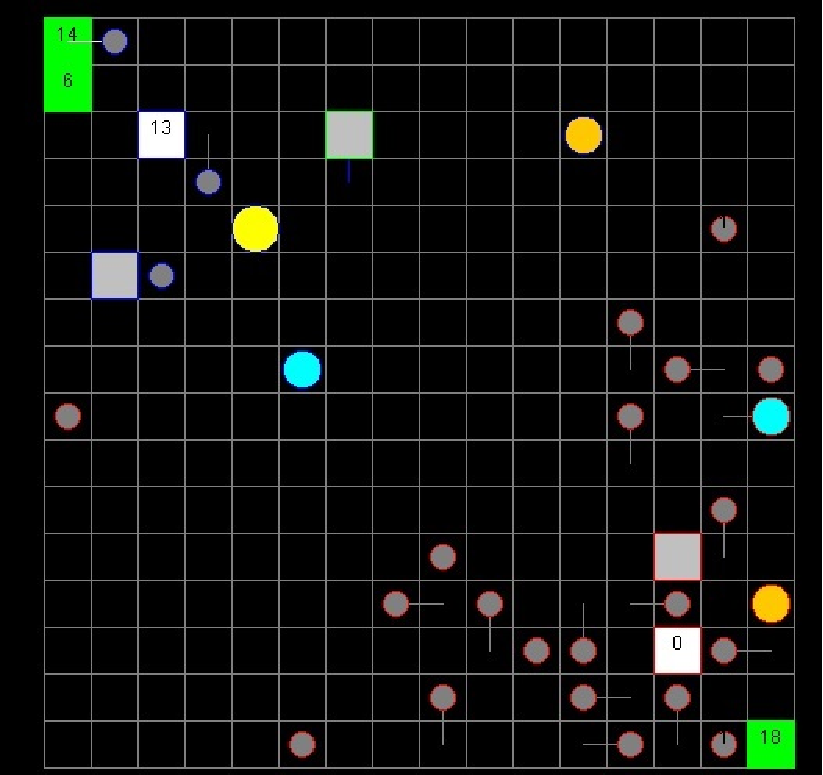
\includegraphics[width=0.5\textwidth]{fig/microrts.pdf}
	\caption{Um exemplo de tela do MicroRTS}
	\label{fig:microrts}
\end{figure} 

\subsection{Unidades e construções}

No MicroRTS existem quatro tipos de unidades no jogo, um trabalhor chamado de \textit{worker} e três unidades de ataque distintas.
A unidade \textit{worker} é responsável por coletar recursos e construir as edificações. 
Esta unidade também consegue lutar mas possui um dano muito baixo.
As unidades de ataque podem apenas atacar, elas custam a mesma quantidade de recursos para serem produzidas, mas suas características são diferentes. 
A unidade \textit{heavy} possui um alto poder de ataque mas sua velocidade é baixa.
Já a unidade \textit{light} possui um baixo poder de ataque mas sua velocidade é maior.
Por fim, a unidade \textit{ranged} consegue atacar de longa distância. 

Para treinar as unidades é preciso ter recursos e edificações. 
A base é a edificação principal, e é responsável pela criação dos \textit{workers}.
Os \textit{workers} coletam os recursos e armazenam na base.
Os recursos são necessários para treinar e construir tudo dentro do jogo. 
O quartel é construído apenas por \textit{workers} e é responsável pela criação das unidades de ataque. 
Todas as unidades e edificações tem um custo em recursos para serem produzidos.

\subsection{Arquitetura}

O MicroRTS conta com cinco classes principais para funcionamento do jogo. 
Cada classe é responsável por um controle dentro do jogo.
As classes \textit{GameState} e \textit{PhysicalGameState} são responsáveis pelo controle das ações das unidades dentro do mapa.
A \textit{UnitTypeTable} é utilizada para associar cada unidade com as suas ações possíveis.
A classe \textit{PhysicalGameStatePanel} é responsável pela interface gráfica.
A classe \textit{GameVisualSimulation} é utilizada para unir todos os componentes do jogo e configurar as informações de mapa, jogadores, humanos ou IAs, e tempo de duração da partida.
O diagrama de classes presente na Figura~\ref{fig:classes} ilustra como as classes se relacionam e seus principais métodos.

\begin{figure}[ht]
	\centering
	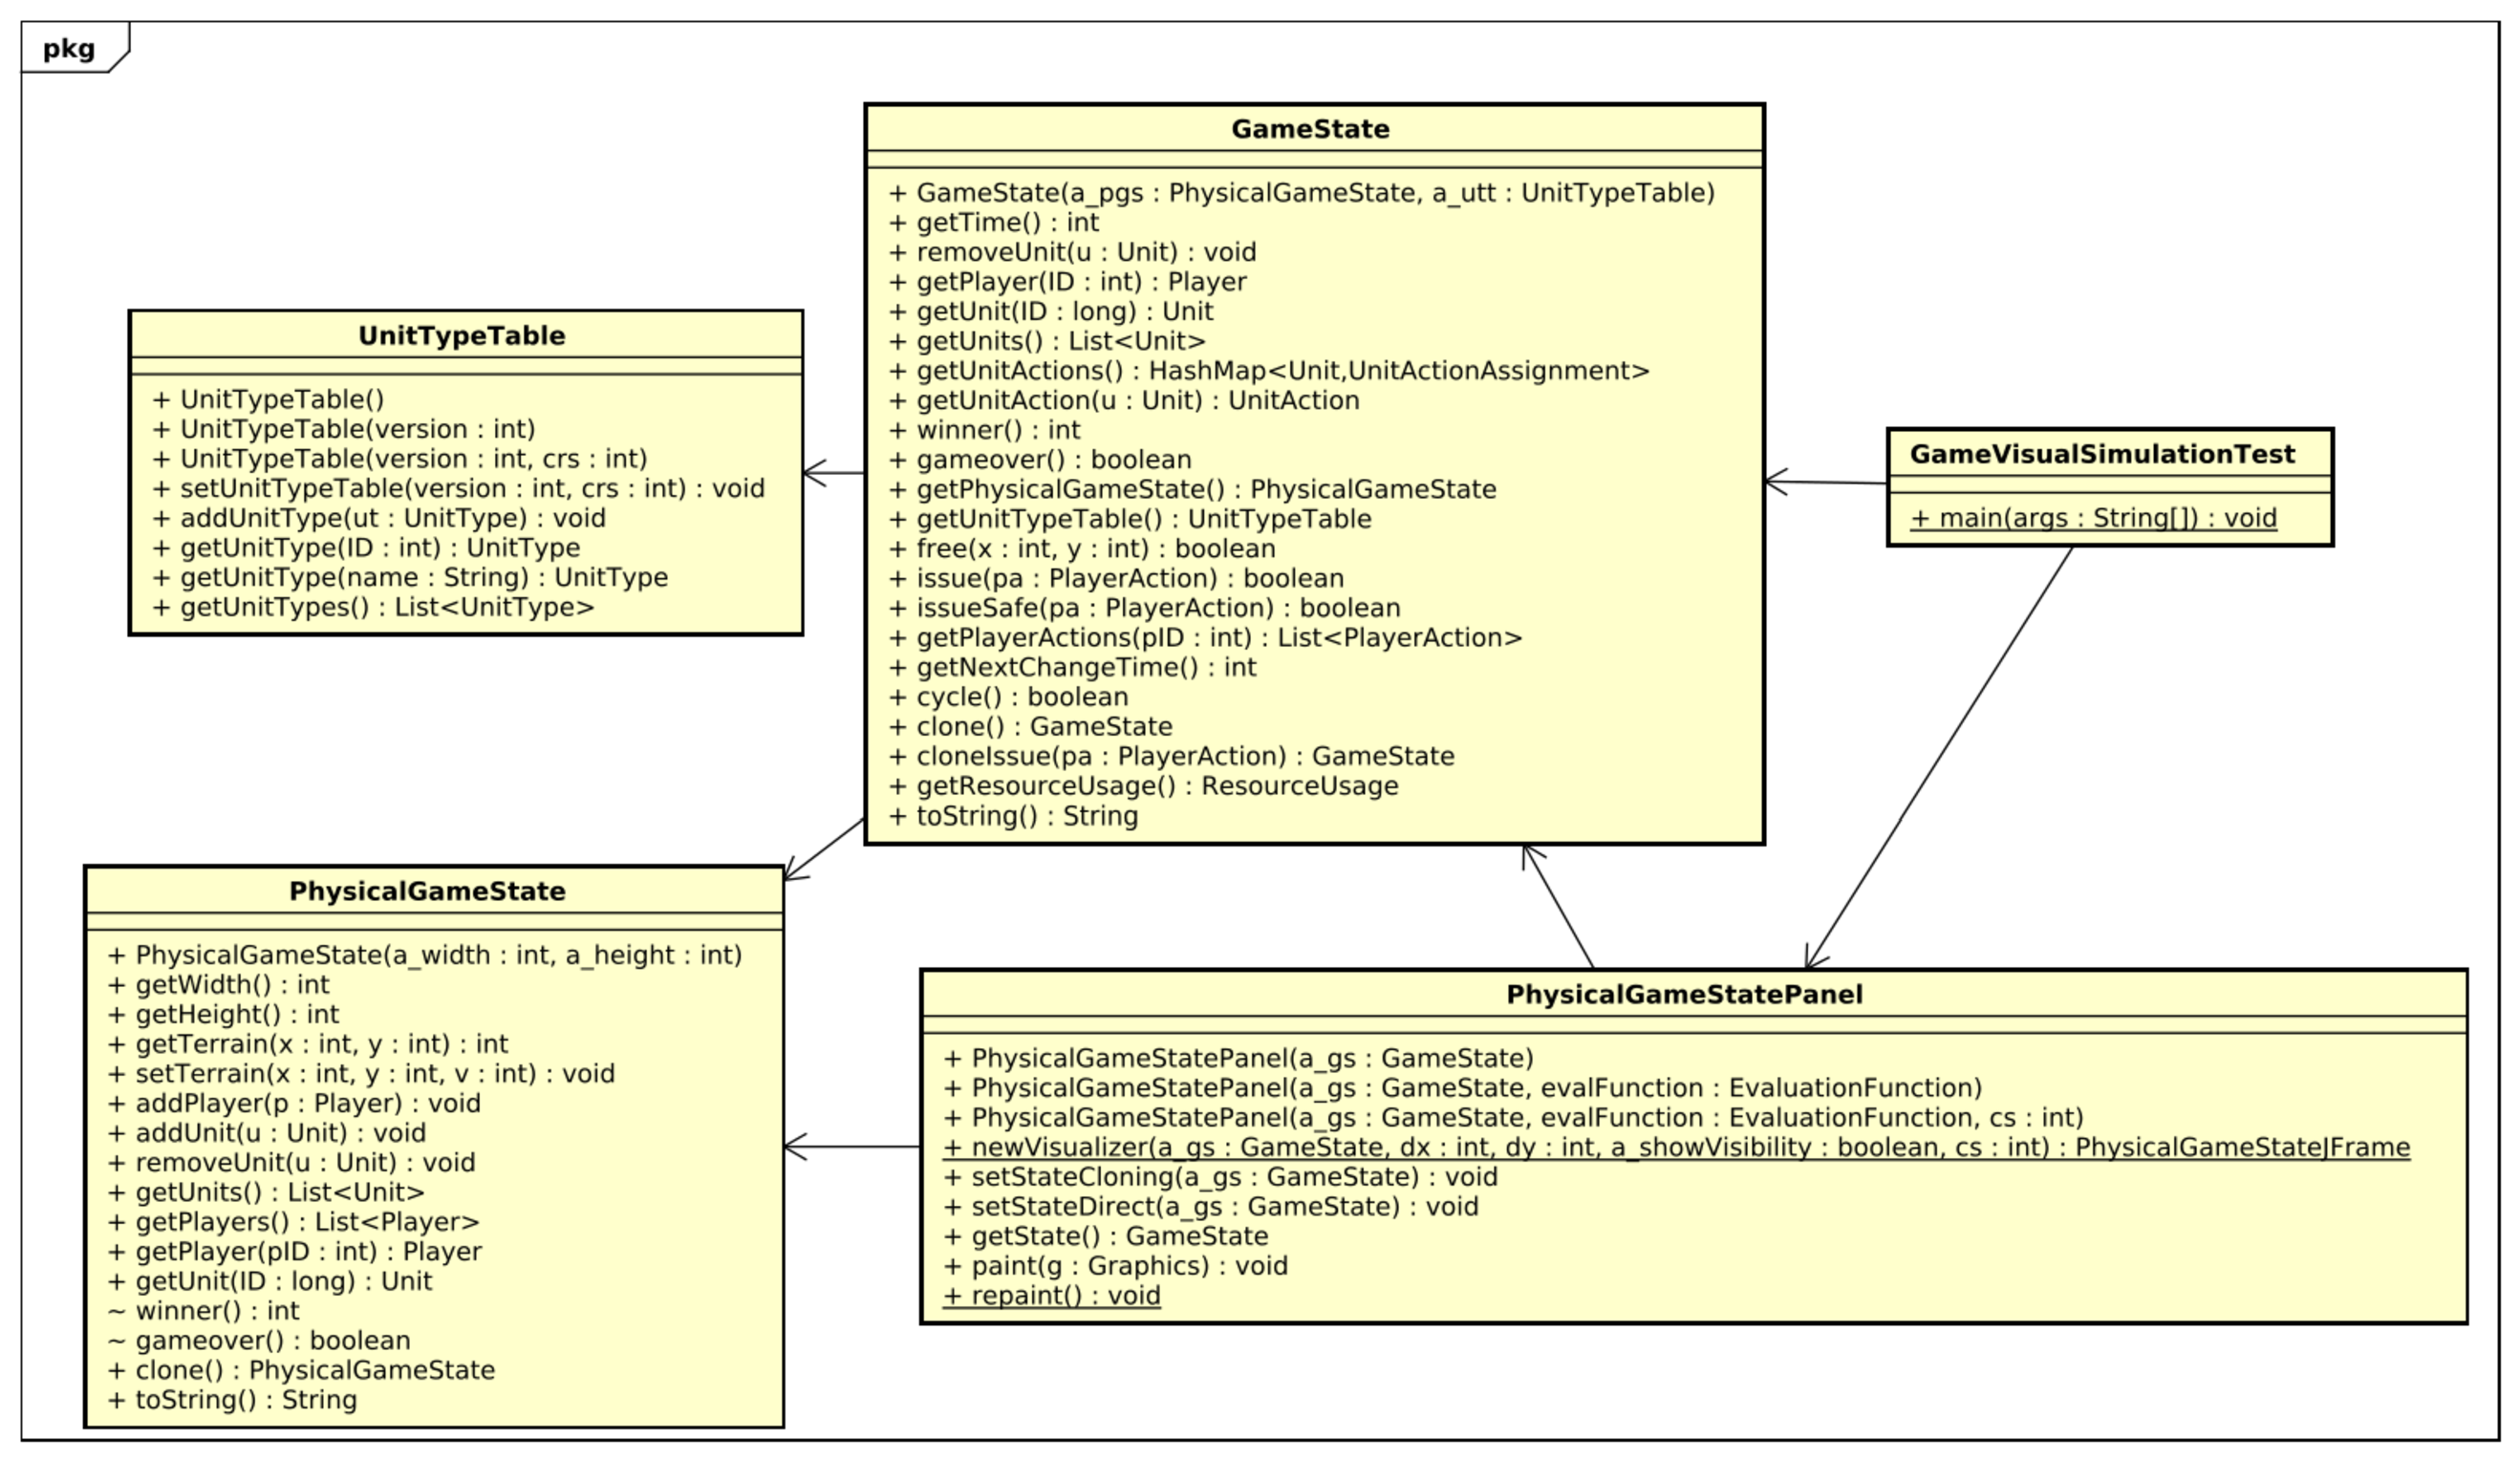
\includegraphics[width=1\textwidth]{fig/classes.pdf}
	\caption{Classes principais do MicroRTS}
	\label{fig:classes}
\end{figure} 

O MicroRTS fornece uma camada de abstração para que se possa utilizar as unidades, sem precisar ter conhecimento de como elas estão estruturadas. 
Essa camada se chama \textit{AbstractionLayerAI}. 
Ela apresenta métodos para treinar unidades, construir edificações, coletar recursos, atacar, e movimentar as unidades. 
Esta camada oferece todos os recursos necessários para que seja implementado um algoritmo de IA.

Todo algoritmo que for implementada no MicroRTS deve conter o método $\mathit{getAction}$.
Este método é responsável por determinar qual ação deve ser realizada pelo algoritmo de IA em determinado momento do jogo.
Cada algoritmo pode assumir o lugar de um jogador no MicroRTS. 
A classe \textit{GameVisualSimulation}, que é responsável por gerenciar a simulação, inicializa os jogadores e a cada período de tempo chama o método para realizar as ações dos jogadores.
A Figura~\ref{fig:sequencia} ilustra o diagrama de sequência do funcionamento do método \texttt{main} da classe \textit{GameVisualSimulation}, e o Algoritmo~\ref{alg:jogo} apresenta o pseudo código do método.
 
A classe primeiro obtém as instâncias dos objetos necessários para a simulação do jogo: esse processo está representado da linha~\ref{alg:jogo:instancia} até a linha~\ref{alg:jogo:instanciaend}.
A linha~\ref{alg:jogo:desenha} é onde o algoritmo chama a classe da interface gráfica para desenhar a tela do jogo.
Após isso, o jogo entra em um laço para que os jogadores façam suas jogadas. As linhas~\ref{alg:jogo:action1} e \ref{alg:jogo:action2} são onde os jogadores escolhem as suas jogadas.
Nas linhas~\ref{alg:jogo:issue1} e \ref{alg:jogo:issue2} as jogadas são testadas para que não haja nenhuma violação quanto as restrições do jogo.
Isso é necessário para que não haja nenhuma inconsistência no jogo, como por exemplo acessar uma posição que não é possível ou ainda construir uma edificação no lugar de outra.
A linha~\ref{alg:jogo:gameover} é responsável por determinar se o jogo acabou.
A linha~\ref{alg:jogo:repaint} desenha a tela novamente com as jogadas executadas.
Assim o laço da linha~\ref{alg:jogo:while} é executado até que o jogo termine com algum vencedor ou quando o tempo de simulação acabar.

\begin{algorithm}
	\caption{Pseudo código da classe \textit{GameVisualSimulation}.}
	\label{alg:jogo}
	\begin{algorithmic}[1]		
		\Function {main}{$String[]$}
		\State $utt = UnitTypeTable()$ \label{alg:jogo:instancia}
		\State $pgs = PhysicalGameState()$
		\State $gs = GameState(pgs, utt)$
		\State $player1 = Player1()$
		\State $player2 = Player2()$ \label{alg:jogo:instanciaend}
		\State $drawScreen()$  \label{alg:jogo:desenha}
		\While{$!gameover() || endTime()$} \label{alg:jogo:while}
			\State $action1 = player1.getAction()$ \label{alg:jogo:action1}
			\State $action2 = player2.getAction()$ \label{alg:jogo:action2}
			\State $issueSafe(action1)$ \label{alg:jogo:issue1}
			\State $issueSafe(action2)$ \label{alg:jogo:issue2}
			\State $gameover = gs.cycle()$ \label{alg:jogo:gameover} 
			\State $repaintScreen()$ \label{alg:jogo:repaint}
		\EndWhile
		\EndFunction
	\end{algorithmic}
\end{algorithm}

\begin{figure}[ht]
	\centering
	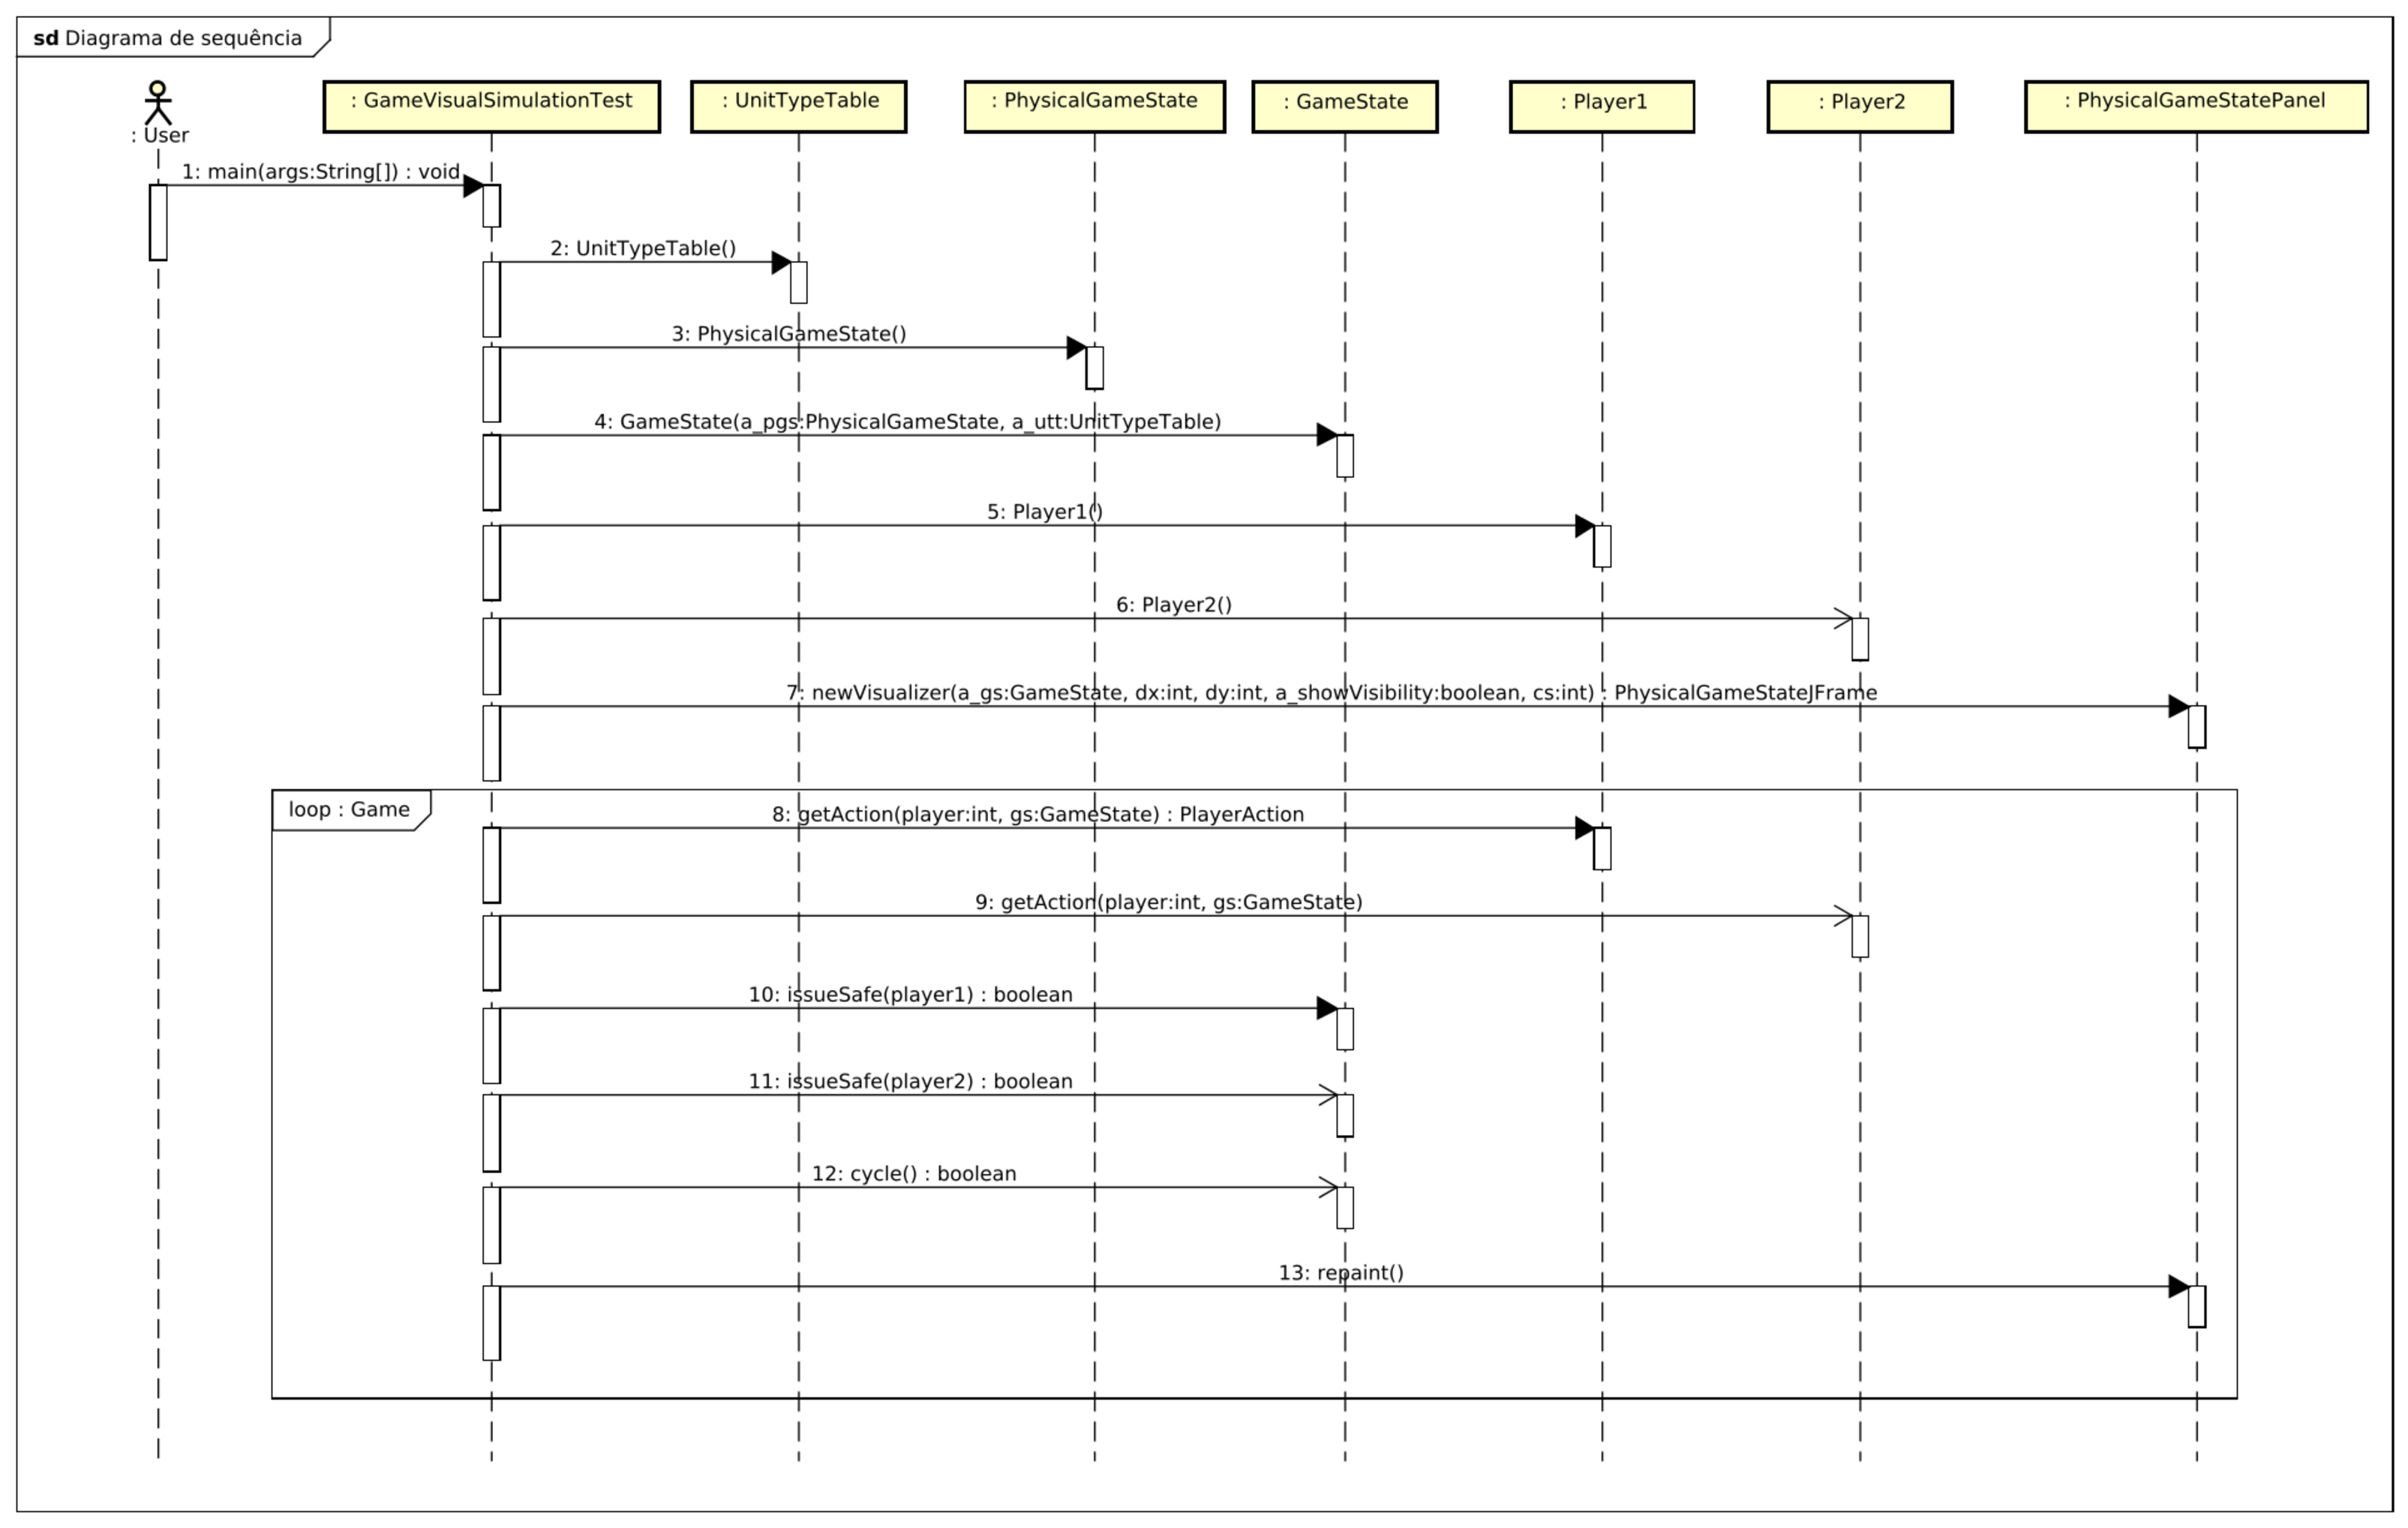
\includegraphics[width=1\textwidth]{fig/diagramaSequencia.pdf}
	\caption{Diagrama de sequência do método \texttt{main} da classe \textit{GameVisualSimulation}}
	\label{fig:sequencia}
\end{figure}

\subsection{Técnicas} \label{sec:tecn}

O MicroRTS possui algumas técnicas que realizam suas jogadas automaticamente já implementadas.
Algumas destas técnicas simulam algum comportamento dentro do jogo, sem ter um algoritmo de IA são chamadas de estratégias hard-coded. 
Estratégias hard-coded consistem em um certo tipo de script com um objetivo inflexível definido em tempo de programação.
No MicroRTS existe algumas estratégias hard-coded implementadas: RandomAI e RandomBiased, LightRush, HeavyRush, RangedRush e WorkerRush.
A RandomAI executa movimentos totalmente aleatórios.
Já a RandomBiasedAI também executa movimentos aleatórios, mas com uma probabilidade maior de realizar três movimentos: ataque, extração de recurso, e criação de tropas.
As demais estratégias são baseadas no mesmo estilo de jogo, mas com unidades de ataque diferentes.
Elas utilizam um \textit{worker} para extrair recursos, e treinam um único tipo de unidade de ataque para atacar. 
As técnicas são chamadas de LightRush, HeavyRush, e RangedRush, elas utilizam as unidades \textit{light}, \textit{heavy}, e \textit{ranged}, respectivamente.
A WorkerRush consiste em ter um \textit{worker} para realizar a extração de recursos mas ao invés de treinar unidades de ataque ela treina outros \textit{workers} para realizar os ataques, isso faz com que a técnica consiga criar muitas unidades de maneira rápida.

Outras técnicas utilizam algum algoritmo de IA para decidir qual ação deve ser realizada, como é o caso das estratégias de Minimax\cite{ontanon2012minimax}, Monte Carlo, e Portfolio Search\footnote{https://github.com/santiontanon/microrts/wiki/Artificial-Intelligence}.
A estratégia de Minimax utiliza o algoritmo de minimax para uma determinada profundidade. A profundidade não é em relação aos turnos, como no algoritmo comum de minimax, mas sim ao tempo disponível para tomar uma decisão.
A estratégia de Monte Carlo verifica todas as ações possíveis para o estado, e simula jogos aleatórios para aquela jogada até um determinado tempo. Uma heurística é utilizada para determinar qual foi a ação que obteve o melhor valor.
Já estratégia de Portfolio Search possui um conjunto de estratégias (o portfólio) e utiliza um algoritmo de busca para decidir qual a melhor estratégia para ser usada em determinado momento. 
O conjunto é composto pelas estratégias Hard-Coded.

O MicroRTS foi escolhido como plataforma para a implementação do algoritmo de AHTN por ser desenvolvido em Java, e também por ter algoritmos de IA já acoplados, isso demonstra a viabilidade de acoplar novas técnicas sem ter conhecimento das estrutura interna do jogo.

\section{Java Simple Hierarchical Ordered Planner 2}\label{sec:jshop}
		
Java Simple Hierarchical Ordered Planner 2 (JSHOP2)~\cite{nauJSHOP2} é um sistema de planejamento independente de domínio baseado em HTN. 
O JSHOP2 foi desenvolvido em Java por Dana Nau e sua equipe de pesquisa.  
O JSHOP2 recebe como entrada uma descrição do domínio e um problema de planejamento.
A descrição do domínio contém a formalização das ações dos agentes, as tarefas e métodos que as decompõem.
O planejador realiza a geração do plano decompondo os métodos até que só restem tarefas primitivas, a Seção~\ref{sec:htnPlanning} explica como é feita a decomposição. 
Na descrição do domínio as tarefas primitivas são descritas como operadores, compostos por um nome de operador, uma lista de precondições que devem ser verdadeiras para a execução do operador, uma lista de elementos que serão removidos do estado, e uma lista de elementos que serão adicionados ao estado. 
Por exemplo, um operador que representa o deslocamento de uma pessoa de um lugar de origem para um lugar de destino, para isso é preciso estar no lugar origem, e assim que a pessoa se locomover ela não está mais neste local e está no local destino. Este exemplo de operador é apresentado a seguir:

\lstset{style=codeStyle}
\begin{lstlisting}[language=lisp]
	(:operator (!move ?from ?to) 
		((at ?from)) ;; Precondition
		((at ?from)) ;; Delete list
		((at ?to))   ;; Add list
	)
\end{lstlisting}

Os métodos são utilizados para decompor tarefas de alto nível para níveis mais baixos. 
No JSHOP2 os métodos são identificados por um nome de método, que é único para cada método. 
Dentro de um método há uma lista de precondições e uma lista de tarefas, que podem ser primitivas ou não primitivas, para quantos casos forem necessários. 
Por exemplo, no problema de ir de um local para outro, se o local destino tem um caminho para o local origem, é possível se locomover para o local, mas se não houver caminho é preciso ir para outra cidade que tenha caminho para o local destino. 
Este exemplo pode ser visto abaixo:

\lstset{style=codeStyle}
\begin{lstlisting}[language=lisp]
	(:method (travel ?from ?to)
		((at ?from) (path ?from ?to)) ;; precondition 
		((!move ?from ?to)) ;; task list
		
		((not (path ?from ?to)) (path ?from ?somewhere)) ;; precondition 
		((!move ?from ?somewhere) (travel ?somewhere ?to)) ;; task list
	)
\end{lstlisting}

A descrição do domínio precisa de um nome. 
O nome é necessário para que o planejador consiga fazer a ligação da descrição do domínio com o problema de planejamento. 
A descrição do domínio com métodos e operadores para o exemplo citado acima ficaria assim:

\lstset{style=codeStyle}
\begin{lstlisting}[language=lisp]
(defdomain move
	(	
		(:operator (!move ?from ?to) 
			((at ?from)) 
			((at ?from))
			((at ?to))
		)
		
		(:method (travel ?from ?to)
			((at ?from) (path ?from ?to))
			((!move ?from ?to))
		
			((not (path ?from ?to)) (path ?from ?somewhere))
			((!move ?from ?somewhere) (travel ?somewhere ?to))
		)    
	)
)
\end{lstlisting}

O problema de planejamento contém as informações do estado do ambiente e qual é o objetivo do agente. 
O estado do ambiente é composto por predicados que são usados nos métodos e operadores, como no exemplo \texttt{at ?x} e \texttt{path ?a ?b}, como é apresentado na Seção~\ref{sec:classicalPlanning}.
O objetivo do agente é expresso por uma ou mais tarefas do domínio, no exemplo \texttt{travel ?from ?to}. Um possível problema de planejamento para o exemplo pode ser o apresentado abaixo:


\begin{lstlisting}[language=lisp]
(defproblem problem move
	( 
		(path PortoAlegre Charqueadas)
		(path Charqueadas SaoJeronimo)
		(at PortoAlegre)
	)
	
	(
		(travel PortoAlegre SaoJeronimo)
	)
)
\end{lstlisting}

O planejador necessita do domínio e do problema para gerar os planos.
O plano gerado inclui o custo para executar este plano, junto com os operadores em ordem que devem ser executados para que o objetivo seja alcançado. 
Caso existam mais planos que levem ao mesmo objetivo, o JSHOP2 apresenta os planos na mesma estrutura.
O plano gerado para o exemplo acima é o seguinte:

\begin{lstlisting}[language=lisp]
[Plan cost: 2.0

(!move portoalegre charqueadas)
(!move charqueadas saojeronimo)
--------------------
]
\end{lstlisting}

O JSHOP2 é um projeto aberto e seu código está disponível\footnote{http://www.cs.umd.edu/projects/shop/} junto com alguns exemplos de domínios e problemas.
O planejador possui funcionalidades, como chamada de funções externas e quantificadores, que podem ser usadas na confecção de domínios~\cite{ilghami2006documentation}.
Entretanto, os exemplos não exploram todas as funcionalidades disponíveis.
Outro ponto negativo do JSHOP2 é o modo como ele está estruturado internamente, há uma forte ligação entre as classes.
O plano gerado não apresenta a informação de quais métodos são foram decompostos para alcançar os operadores.
O JSHOP2 foi escolhido para ser utilizado neste trabalho por estar codificado em Java e ser um planejador reconhecido no meio acadêmico.

No próximo capítulo é apresentada a modelagem do domínio, a implementação do algoritmo de AHTN no MicroRTS e como é feita a tradução do cenário do jogo para um problema de planejamento.

